\subsection{Introduction}

The design is bassed in the following assumptions:

\begin{itemize}
\item Design wall with pinned base and pinned top.
\item Neglect corner regions (wall spans one-way only).
\item Top slab is in place and has achieved full strength prior to backfilling.
\item Vehicular traffic around the building is represented by a uniform load of $250\ psf$ ($11.97\ kN/m^2$).
\item The vertical response of the soil calculated using a Winkler model with a subgrade reaction module of set of 200 pounds per cubic inch ($54.29 \times 10^6\ N/m^3$).
\item Water table deep below structure.
\end{itemize}

\subsection{Load determination}

\subsubsection{Self weight}
The self weight of the reinforced concrete is calculated from its density: $2500\ kg/m^3$.

\subsubsection{Axial loads from building}
The loads transferred by the top slab to the wall are as follows:

\begin{center}
  \begin{tabular}{|l|l|r|r|}
\hline
\textbf{Building} & \textbf{Load} & \textbf{Phase 1} & \textbf{Phase 2}\\
\textbf{side} &  & (kN/m) & (kN/m)\\
\hline
North & SnowL & 10.06 & 10.06\\
North & LiveL & 21.67 & 21.67\\
North & Wind\_NS & -15.12 & -15.12\\
North & Wind\_WE & -1.33 & -1.33\\
North & DeadL & 31.54 & 31.54\\
\hline
South & SnowL & 8.04 & 16.08\\
South & LiveL & 14.22 & 28.44\\
South & Wind\_NS & 4.97 & 9.95\\
South & Wind\_WE & -0.23 & -0.46\\
South & DeadL & 20.58 & 41.15\\
\hline
East & SnowL & 11.96 & 11.96\\
East & LiveL & 23.75 & 23.75\\
East & Wind\_NS & -0.07 & -0.07\\
East & Wind\_WE & 12.97 & 12.97\\
East & DeadL & 30.87 & 30.87\\
\hline
West & SnowL & 15.02 & 15.02\\
West & LiveL & 27.15 & 27.15\\
West & Wind\_NS & -0.20 & -0.20\\
West & Wind\_WE & -13.20 & -13.20\\
West & DeadL & 29.81 & 29.81\\
\hline
\end{tabular}
\end{center}

\subsubsection{Earth pressure}
The soil pressure over the wall has been calculated using the lateral pressure at rest with a coefficient $K_0= 0.5$.

\subsection{Stem dimensions and reinforcement}
The thickness and the reinforcement for the walls are indicated in the table \ref{tb_concrete_wall_reinforcing_schedule}.

\begin{table}
    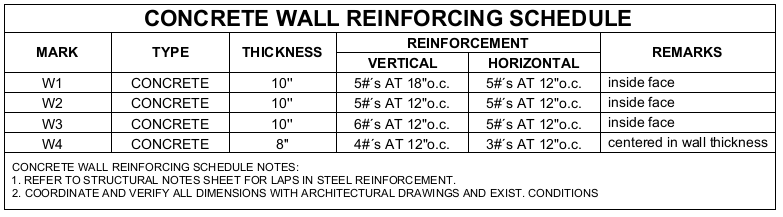
\includegraphics[width=\linewidth]{figures/concrete_wall_reinforcing_schedule.png}
    \caption{Concrete walls reinforcing schedule}\label{tb_concrete_wall_reinforcing_schedule}
\end{table}

\subsubsection{Wall types}
For analysis purposes we have considered the following wall types:

\begin{center}
  \begin{tabular}{|l|r|}
    \hline
    \textbf{Wall} & \textbf{Stem height (m)} \\
    \hline
T1 & 3.15\\
T2 & 2.74\\
T3 & 3.53\\
T4 & 3.12\\
T5 & 2.51\\
T6 & 3.43\\
    \hline
  \end{tabular}
\end{center}


